%%%%%%%%%%%%%%%%%%%%%%%%%%%%%%%%%%%%%%%%%
% FRI Data Science_report LaTeX Template
% Version 1.0 (28/1/2020)
% 
% Jure Demšar (jure.demsar@fri.uni-lj.si)
%
% Based on MicromouseSymp article template by:
% Mathias Legrand (legrand.mathias@gmail.com) 
% With extensive modifications by:
% Antonio Valente (antonio.luis.valente@gmail.com)
%
% License:
% CC BY-NC-SA 3.0 (http://creativecommons.org/licenses/by-nc-sa/3.0/)
%
%%%%%%%%%%%%%%%%%%%%%%%%%%%%%%%%%%%%%%%%%


%----------------------------------------------------------------------------------------
%	PACKAGES AND OTHER DOCUMENT CONFIGURATIONS
%----------------------------------------------------------------------------------------
\documentclass[fleqn,moreauthors,10pt]{ds_report}
\usepackage[english]{babel}

\graphicspath{{fig/}}




%----------------------------------------------------------------------------------------
%	ARTICLE INFORMATION
%----------------------------------------------------------------------------------------

% Header
\JournalInfo{FRI Natural language processing course 2021}

% Interim or final report
\Archive{Project report} 
%\Archive{Final report} 

% Article title
\PaperTitle{Parameter-Efficient Fine-Tuning of Language Models for Slovene} 

% Authors (student competitors) and their info
\Authors{Camile Lenderling, Manfred González, and Joaquín Figueira}

% Advisors
\affiliation{\textit{Advisors: Slavko Žitnik}}

% Keywords
\Keywords{LLM, LM, PEFT, NLP, Slovene, LoRA, BitFit, p-tuning}
\newcommand{\keywordname}{Keywords}


%----------------------------------------------------------------------------------------
%	ABSTRACT
%----------------------------------------------------------------------------------------

\Abstract{
This work adapts and evaluates several parameter efficient finetuning techniques (PEFT) for large language models pre-trained on the Slovenian language. It focuses on methods based on LoRA, bias tuning and prefix tuning. The performance of these methods is assessed with SloBENCH, and evaluation framework for the Slovenian language, and focuses on natural language understanding (NLU) and machine translation tasks (MT). Results are compared with previous submissions to the evaluation framework to determine the relative effectiveness of PEFT methods in a Slovenian linguistic context.  
}

%----------------------------------------------------------------------------------------

\begin{document}

% Makes all text pages the same height
\flushbottom 

% Print the title and abstract box
\maketitle 

% Removes page numbering from the first page
\thispagestyle{empty} 

%----------------------------------------------------------------------------------------
%	ARTICLE CONTENTS
%----------------------------------------------------------------------------------------

\section*{Introduction}

    Large language models and, by extension, language models (LM) in general are becoming ubiquitous in the current technological landscape. As such, the amount of tasks and applications that are being performed by, or with the help of these models is continuously growing. Until recently, LMs were built for specific taks, but with the advent of LLMs this has become both unnecessary, as models are complex enough now that they can perform multiple tasks well out-of-the-box, and unfeasible, as building these models takes an enormous amount of computational resources. However, if one is to achieve the optimal performance on a given task or expand the capabilities of a LM, some adaptations of the model are in order.
    
    These adaptations usually come in the form of a process called finetuning, in which the parameters of an already pretrained language model (PLM) are fitted for the specific task we want to achieve. Nonetheless, given the massive amount of parameters in modern LLMs, full finetuning (FFT) of the weights of a model is usually too computationally prohibitive for most applications. As a result, in the recent years many techniques have been developed to efficiently tune LMs, focusing specifically in reducing the amount of parameters that actually have to be trained (a comprehensive review of this techniques can be found on \cite{survey}). These are usually referred to with the umbrella term parameter efficient fine-tuning techniques (PEFT) and are mainly based on the Lottery Ticket Hypothesis, which states that ``large models are needed in pretraining only to induce (in high probability) the existence of sub-networks initialized with the correct inductive bias for learning.''. In other words, that PLMs already contain the capacity and linguistic ``knowledge'' to perform a wide variety of tasks, but this abilities need to be accentuated through the proper learning stimulus that induces the use of the correct sub-networks when performing a particular task. 

    The purpose of this work is precisely to adapt and evaluate several PEFT techniques with a focus on the Slovenian language. To cover a wide range of approaches the analyzed techniques will span different families: LoRA\cite{hu2022lora} and its derivatives, bias tuning\cite{bitfit} and soft prompt based techniques. As a base model for analysis the SloBERT LM will be used, which is a BERT model optimized for Slovenian. For performance assessment the techniques will be assessed on multiple NLP tasks focused on natural language understanding (NLU) and machine translation (MT) using some of the NLP benchmarks provided in the Slobench Slovenian evaluation framework, mainly the Slovene SuperGLUE and Machine Translation (SLO - ENG) benchmarks. A final analysis will also be provided comparing the results of the fine-tuned models with the metrics from previous submissions to Slobench of the same benchmarks. 


%------------------------------------------------

\section*{Methods}

The field of adapting large language models (LLMs) for specific tasks has seen significant advancements with the introduction of Low-Rank Adaptation (LoRA). Hu et al.~\cite{hu2022lora} pioneered this approach by freezing the pre-trained model weights and integrating trainable rank decomposition matrices into the Transformer architecture. This method not only substantially reduces the number of trainable parameters required for downstream tasks but also lessens the GPU memory requirements, thereby enabling comparable or superior model quality with notable efficiency. The provision of a package to facilitate the integration of LoRA with PyTorch models, including implementations for popular models like RoBERTa, DeBERTa, and GPT-2, marks a significant contribution to the field.

Further enhancing the parameter efficiency of fine-tuning PLMs, Zhang et al.~\cite{zhang2023increlora} introduced IncreLoRA, an incremental parameter allocation method that judiciously adds trainable parameters based on the importance scores of each module. This approach, distinguished from structured pruning methods, not only improves parameter efficiency but also incorporates early learning and restart warmup techniques to bolster training effectiveness and stability. The method demonstrated superior parameter efficiency and model performance, particularly in low-resource settings, through rigorous experiments on the GLUE benchmark.

On the deployment front, Xu et al.~\cite{xu2023qalora} proposed the Quantization-Aware Low-Rank Adaptation (QA-LoRA) algorithm, aimed at the efficient deployment of LLMs on edge devices. By introducing group-wise operators, QA-LoRA enhances the quantization flexibility while streamlining adaptation, enabling the integration of quantized LLM and auxiliary weights without compromising accuracy. This method stands out by allowing for low-bit inference directly, overcoming the limitations of previous approaches like QLoRA and facilitating faster model deployment on resource-constrained devices.

Lastly, the scalability and efficiency of serving multiple LoRA adapters derived from a base model have been addressed by Sheng et al.~\cite{sheng2023slora} through the introduction of S-LoRA. This system, designed for scalable serving, significantly improves throughput and the capacity to serve numerous task-specific fine-tuned models by employing a unified memory management approach and optimized computation strategies. Complementing these efforts, Gao et al.~\cite{gao2024higher} introduced MoE-LoRA with Layer-wise Expert Allocation (MoLA), which optimizes the allocation of LoRA experts across different layers of the Transformer model, thereby enhancing model efficiency and performance across various NLP tasks. These advancements collectively signify a leap forward in the efficient adaptation, deployment, and serving of LLMs, paving the way for broader application and innovation in the domain.

\subsection*{Bias update}

BitFit\cite{bitfit} is the first recorded technique to have implemented a sparse-finetunning of LMs using only the bias parameters and it falls under the category of partial fine-tuning according to Xu et. al.'s taxonomy\cite{survey}. The main mechanism of the technique is simple: during fine-tuning an LM on a particular task update only the bias parameters of the model's encoder layers. These parameters account for only a small fraction of all the parameters of the model (0.1\% in the case of BERT). Additionally, the authors found that fitting only a small subset of these bias parameters (mainly the bias of the query encoders of the attention heads and the biases of one of the layers of the MLP inside of the encoder layer) leads to almost no performance drop and modifies only 0.04\% of the parameters. According to Xu et al. \cite{survey} the technique achieves relatively great results with only a fraction of the memory footprint of other PEFTs. These promising results, combined with the existence of multiple pre-packaged implementations of the technique, led us to choose it as one of the subjects of analysis of this work.  

The findings of the initial BitFit paper were further expanded in the works of Lawton et al.\cite{us-bitfit} using neural architecture search (NAS), more specifically, iterative network pruning. The core idea of the method is to iteratively fine-tune the model using BitFit\footnote{The authors also fine-tuned the models using LoRA, but that falls outside of the scope of this analysis.} and then prune it's bias parameters according to a criteria based on the first order approximation of the loss that results from eliminating certain parameters from the network. The authors found that the resulting network architectures could maintain good performance with a large portion of their bias parameters pruned, further solidifying the findings in the initial BitFit paper that only a relatively small number of bias parameters are responsible for the fine-tuned performance. Unfortunately, there is no code or implementation freely available to replicate the results of this technique in our work.


\iffalse
- Sparse-finetunning technique
- Only updates bias-terms of attention modules
- Main hypothesis: finetunning is about exposing knowledge induced by language-modeling training?
- Trains only 0.1% of parameters
    - Even Lower if we only train the bias of the query encoders and third layer of FF. In this case it trains 0.04% of parameters.
- \textbf{Results:}
    - Achieves similar performance than FFT in the Glue benchmark using LargeBert (question: finetunes for each task?), and similar or better performance than other comparable techniques at the time with only a fraction of the parameters they use
    - BitFit is more data efficient than FFT: it achieves better results then FFT in small-medium data regimes

\textbf{Lottery Ticket Hypothesis}

(Frankle and Carbin, 2019; Chen et al., 2020; Prasanna et al., 2020) 

\textit{Include in introduction}

The conjecture that large models are needed in pretraining only to induce (in high probability) the existing of sub-networks initialized with the correct inductive bias for learning.

\fi

\subsection*{Soft prompts}
Soft prompts, represent various methods to efficiently adapt LLMs for down-stream tasks without altering the underlying model architecture or weights. This technique involves appending a sequence of tunable tokens, or "soft prompts," to the input of the model. During fine-tuning, these tokens are optimized to guide the model towards generating the desired task-specific output. Two prominent methods for implementing soft prompts are prompt tuning and prefix tuning. 

\subsubsection*{Prompt tuning}
Prompt tuning introduces a set of $\ell$ learnable tokens (soft prompts), denoted as $P =  \{P_1, P_2, \dots P_\ell$\},  and concatenates these tokens to beginning of the input to the model $X \in \mathbb{R}^{n\times d}$ to form $\hat{X} \in \mathbb{R}^{(n + \ell) \times d}$. Throughout the fine-tuning process, only the parameters associated with the prompt tokens $P$ are adjusted via gradient descent, while the pre-trained model parameters are kept fixed. Hence, the length of the prompt and the dimensionality of the token embeddings determine the parameter cost for fine-tuning.~\cite{prompt_tuning} 

\subsubsection*{Prefix-tuning}
Prefix-tuning introduces the idea of appending a set of soft prompts $P =  \{P_1, P_2, \dots P_\ell$\}, not to the input layer but to the hidden states within the multi-head attention layers of the model. This is different from prompt tuning, which concatenates  soft prompts directly to the input. To promote stability during training, a feed-forward network (FFN) is used to parameterize these soft prompts. During fine-tuning, two distinct sets of prefix vectors, $\hat{P}_K$ and $\hat{P_V}$, are concatenated to the attention layer's original key ($K$) and value ($V$) vectors, respectively. Hence, the only parameters that require optimization are those of $\hat{P}_K$, $\hat{P_V}$, and the FFN. Once the model is fine-tuned, the FFN is no longer needed, and only the optimized key and value prefix vectors are kept for model inference.~\cite{prefix_tuning}


\section{Proposed Methodology}
Our proposed methodology is as follows (sketch):
\begin{enumerate}
    \item Select and preprocess datasets from the SloBench framework.
    \item Format data for NLP tasks using appropriate tokenizers for SloBERTa and other multilingual LMs.
    \item Establish performance baselines for the untuned SloBERTa and other selected multilingual LLMs.
    \item Using HuggingFace's PEFT library, apply various prominant PEFT techniques such as LoRa, Bias Tuning, and Soft Prompts to fine-tune the LMs on different downstream tasks.
    \item Use SloBench to evaluate fine-tuned models, comparing performance across different PEFT methods and NLP tasks.
\end{enumerate}


% \subsection*{Equations}

% You can write equations inline, e.g. $\cos\pi=-1$, $E = m \cdot c^2$ and $\alpha$, or you can include them as separate objects. The Bayes’s rule is stated mathematically as:

% \begin{equation}
% 	P(A|B) = \frac{P(B|A)P(A)}{P(B)},
% 	\label{eq:bayes}
% \end{equation}

% where $A$ and $B$ are some events. You can also reference it -- the equation \ref{eq:bayes} describes the Bayes's rule.

% \subsection*{Lists}

% We can insert numbered and bullet lists:

% % the [noitemsep] option makes the list more compact
% \begin{enumerate}[noitemsep] 
% 	\item First item in the list.
% 	\item Second item in the list.
% 	\item Third item in the list.
% \end{enumerate}

% \begin{itemize}[noitemsep] 
% 	\item First item in the list.
% 	\item Second item in the list.
% 	\item Third item in the list.
% \end{itemize}

% We can use the description environment to define or describe key terms and phrases.

% \begin{description}
% 	\item[Word] What is a word?.
% 	\item[Concept] What is a concept?
% 	\item[Idea] What is an idea?
% \end{description}


% \subsection*{Random text}

% This text is inserted only to make this template look more like a proper report. Lorem ipsum dolor sit amet, consectetur adipiscing elit. Etiam blandit dictum facilisis. Lorem ipsum dolor sit amet, consectetur adipiscing elit. Interdum et malesuada fames ac ante ipsum primis in faucibus. Etiam convallis tellus velit, quis ornare ipsum aliquam id. Maecenas tempus mauris sit amet libero elementum eleifend. Nulla nunc orci, consectetur non consequat ac, consequat non nisl. Aenean vitae dui nec ex fringilla malesuada. Proin elit libero, faucibus eget neque quis, condimentum laoreet urna. Etiam at nunc quis felis pulvinar dignissim. Phasellus turpis turpis, vestibulum eget imperdiet in, molestie eget neque. Curabitur quis ante sed nunc varius dictum non quis nisl. Donec nec lobortis velit. Ut cursus, libero efficitur dictum imperdiet, odio mi fermentum dui, id vulputate metus velit sit amet risus. Nulla vel volutpat elit. Mauris ex erat, pulvinar ac accumsan sit amet, ultrices sit amet turpis.

% Phasellus in ligula nunc. Vivamus sem lorem, malesuada sed pretium quis, varius convallis lectus. Quisque in risus nec lectus lobortis gravida non a sem. Quisque et vestibulum sem, vel mollis dolor. Nullam ante ex, scelerisque ac efficitur vel, rhoncus quis lectus. Pellentesque scelerisque efficitur purus in faucibus. Maecenas vestibulum vulputate nisl sed vestibulum. Nullam varius turpis in hendrerit posuere.


% \subsection*{Figures}

% You can insert figures that span over the whole page, or over just a single column. The first one, \figurename~\ref{fig:column}, is an example of a figure that spans only across one of the two columns in the report.

% \begin{figure}[ht]\centering
% 	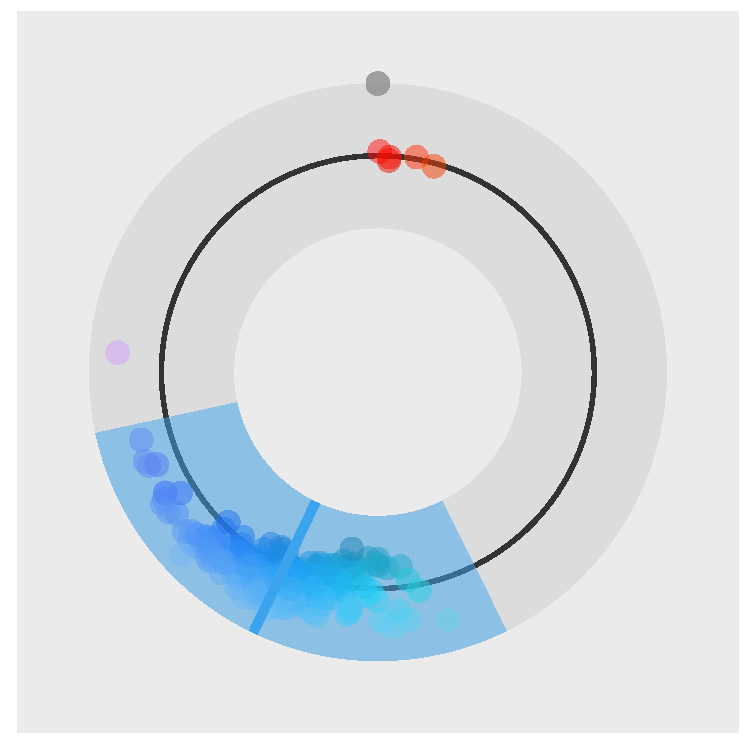
\includegraphics[width=\linewidth]{single_column.pdf}
% 	\caption{\textbf{A random visualization.} This is an example of a figure that spans only across one of the two columns.}
% 	\label{fig:column}
% \end{figure}

% On the other hand, \figurename~\ref{fig:whole} is an example of a figure that spans across the whole page (across both columns) of the report.

% % \begin{figure*} makes the figure take up the entire width of the page
% \begin{figure*}[ht]\centering 
% 	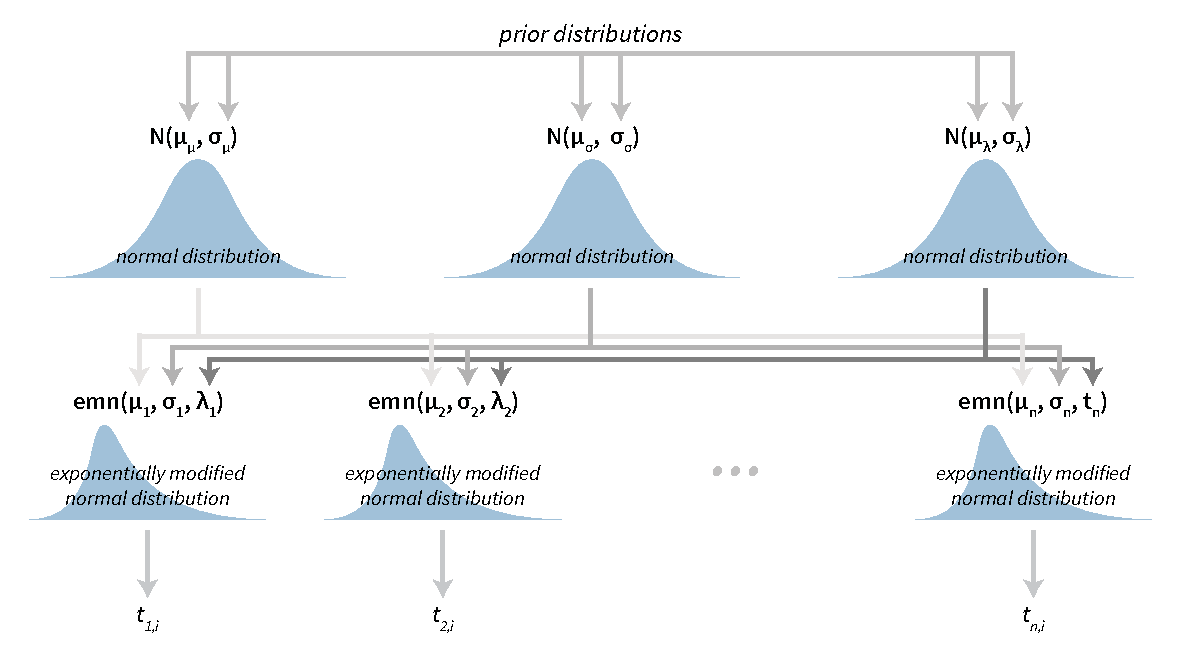
\includegraphics[width=\linewidth]{whole_page.pdf}
% 	\caption{\textbf{Visualization of a Bayesian hierarchical model.} This is an example of a figure that spans the whole width of the report.}
% 	\label{fig:whole}
% \end{figure*}


% \subsection*{Tables}

% Use the table environment to insert tables.

% \begin{table}[hbt]
% 	\caption{Table of grades.}
% 	\centering
% 	\begin{tabular}{l l | r}
% 		\toprule
% 		\multicolumn{2}{c}{Name} \\
% 		\cmidrule(r){1-2}
% 		First name & Last Name & Grade \\
% 		\midrule
% 		John & Doe & $7.5$ \\
% 		Jane & Doe & $10$ \\
% 		Mike & Smith & $8$ \\
% 		\bottomrule
% 	\end{tabular}
% 	\label{tab:label}
% \end{table}


% \subsection*{Code examples}

% You can also insert short code examples. You can specify them manually, or insert a whole file with code. Please avoid inserting long code snippets, advisors will have access to your repositories and can take a look at your code there. If necessary, you can use this technique to insert code (or pseudo code) of short algorithms that are crucial for the understanding of the manuscript.

% \lstset{language=Python}
% \lstset{caption={Insert code directly from a file.}}
% \lstset{label={lst:code_file}}
% \lstinputlisting[language=Python]{code/example.py}

% \lstset{language=R}
% \lstset{caption={Write the code you want to insert.}}
% \lstset{label={lst:code_direct}}
% \begin{lstlisting}
% import(dplyr)
% import(ggplot)

% ggplot(diamonds,
% 	   aes(x=carat, y=price, color=cut)) +
%   geom_point() +
%   geom_smooth()
% \end{lstlisting}

%------------------------------------------------

\section*{Results}

% Use the results section to present the final results of your work. Present the results in a objective and scientific fashion. Use visualisations to convey your results in a clear and efficient manner. When comparing results between various techniques use appropriate statistical methodology.

% \subsection*{More random text}

% This text is inserted only to make this template look more like a proper report. Lorem ipsum dolor sit amet, consectetur adipiscing elit. Etiam blandit dictum facilisis. Lorem ipsum dolor sit amet, consectetur adipiscing elit. Interdum et malesuada fames ac ante ipsum primis in faucibus. Etiam convallis tellus velit, quis ornare ipsum aliquam id. Maecenas tempus mauris sit amet libero elementum eleifend. Nulla nunc orci, consectetur non consequat ac, consequat non nisl. Aenean vitae dui nec ex fringilla malesuada. Proin elit libero, faucibus eget neque quis, condimentum laoreet urna. Etiam at nunc quis felis pulvinar dignissim. Phasellus turpis turpis, vestibulum eget imperdiet in, molestie eget neque. Curabitur quis ante sed nunc varius dictum non quis nisl. Donec nec lobortis velit. Ut cursus, libero efficitur dictum imperdiet, odio mi fermentum dui, id vulputate metus velit sit amet risus. Nulla vel volutpat elit. Mauris ex erat, pulvinar ac accumsan sit amet, ultrices sit amet turpis.

% Phasellus in ligula nunc. Vivamus sem lorem, malesuada sed pretium quis, varius convallis lectus. Quisque in risus nec lectus lobortis gravida non a sem. Quisque et vestibulum sem, vel mollis dolor. Nullam ante ex, scelerisque ac efficitur vel, rhoncus quis lectus. Pellentesque scelerisque efficitur purus in faucibus. Maecenas vestibulum vulputate nisl sed vestibulum. Nullam varius turpis in hendrerit posuere.

% Nulla rhoncus tortor eget ipsum commodo lacinia sit amet eu urna. Cras maximus leo mauris, ac congue eros sollicitudin ac. Integer vel erat varius, scelerisque orci eu, tristique purus. Proin id leo quis ante pharetra suscipit et non magna. Morbi in volutpat erat. Vivamus sit amet libero eu lacus pulvinar pharetra sed at felis. Vivamus non nibh a orci viverra rhoncus sit amet ullamcorper sem. Ut nec tempor dui. Aliquam convallis vitae nisi ac volutpat. Nam accumsan, erat eget faucibus commodo, ligula dui cursus nisi, at laoreet odio augue id eros. Curabitur quis tellus eget nunc ornare auctor.


%------------------------------------------------

\section*{Discussion}

% Use the Discussion section to objectively evaluate your work, do not just put praise on everything you did, be critical and exposes flaws and weaknesses of your solution. You can also explain what you would do differently if you would be able to start again and what upgrades could be done on the project in the future.


%------------------------------------------------

\section*{Acknowledgments}

% Here you can thank other persons (advisors, colleagues ...) that contributed to the successful completion of your project.


%----------------------------------------------------------------------------------------
%	REFERENCE LIST
%----------------------------------------------------------------------------------------
\bibliographystyle{unsrt}
\bibliography{report}


\end{document}